\chapter{Gouvernance et management d'entreprise}
\label{ch:governance}

\section{Introduction}

Les plateformes de place de marché durables exigent plus qu'une vision produit : elles nécessitent une gouvernance institutionnelle qui alloue l'autorité, gère les risques et aligne les incitations entre les fonctions. Ce chapitre décrit le fonctionnement de MABRID en tant qu'entreprise---structure organisationnelle, prise de décision, planification stratégique, gestion opérationnelle, stratégie entrepreneuriale et mesure de la performance---formant l'épine dorsale managériale qui soutient les programmes de sécurité et de conformité.

\section{Gouvernance organisationnelle}

\subsection{Principes de gouvernance d'entreprise}

MABRID adopte des principes alignés sur les orientations de gouvernance d'entreprise de l'OCDE, adaptés aux entreprises en phase de démarrage \parencite{oecd2015governance} : responsabilité de la direction envers les parties prenantes, transparence des risques matériels, allocation responsable des ressources et supervision indépendante des questions d'audit et de sécurité lorsque cela est possible.

\subsection{Conseil d'administration et supervision exécutive}

À maturité, la gouvernance comprend un conseil d'administration (ou un conseil consultatif avant la série A) doté de chartes définies. La direction exécutive comprend le directeur général, le directeur des opérations, le directeur de la technologie (gouvernance du risque technologique, sans détail d'implémentation), le directeur de la sécurité de l'information, le directeur juridique et conformité, et le responsable de la confiance et de la sécurité.

\figureplaceholder{H}{figures/ch02-org-chart.pdf}{0.95}{Structure illustrative de gouvernance organisationnelle}

\subsection{Trois lignes de défense}

La gestion des risques suit le modèle des trois lignes \parencite{iia2017three} :
\begin{enumerate}
  \item \textbf{Première ligne :} Unités métier propriétaires du risque opérationnel (opérations de la place de marché, réussite des vendeurs).
  \item \textbf{Deuxième ligne :} Fonctions risque, conformité et sécurité définissant les normes et surveillant leur application.
  \item \textbf{Troisième ligne :} Audit interne (ou audit externe en phase initiale) fournissant une assurance indépendante.
\end{enumerate}

\section{Structure de l'entreprise et rôles}

\subsection{Départements fonctionnels}

Le tableau~\ref{tab:roles} résume les responsabilités principales. Des matrices RACI (Responsable, Accountable, Consulté, Informé) doivent être maintenues pour les processus critiques, notamment la réponse aux incidents, les mises à jour de politiques et l'intégration des fournisseurs.

\begin{table}[H]
  \centering
  \caption{Rôles exécutifs et principaux domaines de responsabilité}
  \label{tab:roles}
  \begin{tabularx}{\textwidth}{@{}lX@{}}
    \toprule
    \textbf{Rôle} & \textbf{Responsabilité} \\
    \midrule
    CEO & Stratégie, relations investisseurs, engagement réglementaire \\
    COO & Opérations, intégration des vendeurs, SLA de support \\
    CISO & Programme de sécurité, acceptation des risques, commandement des incidents \\
    CLO & Politiques juridiques, liaison CNDP, gouvernance contractuelle \\
    Responsable confiance et sécurité & Modération, prévention de la fraude, normes communautaires \\
    CFO & Contrôles financiers, gouvernance des coûts cloud, économie unitaire \\
    \bottomrule
  \end{tabularx}
\end{table}

\subsection{Cadre de prise de décision}

Les décisions stratégiques (expansion de marché, partenariats majeurs, investissements en certification) requièrent l'approbation du conseil d'administration ou du comité exécutif. Les décisions opérationnelles suivent des limites d'autorité déléguée documentées dans un manuel de gouvernance. Les dérogations de sécurité requièrent l'approbation du CISO avec des plans de remédiation à échéance définie.

\section{Planification stratégique}

\subsection{Horizon de planification}

MABRID emploie des plans opérationnels glissants sur 12 mois imbriqués dans un plan stratégique triennal. Les revues d'affaires trimestrielles évaluent la performance des KPI, la dynamique concurrentielle et les évolutions réglementaires.

\subsection{Analyse SWOT}

\begin{table}[H]
  \centering
  \caption{Analyse SWOT stratégique pour MABRID}
  \label{tab:swot}
  \begin{tabularx}{\textwidth}{@{}XX@{}}
    \toprule
    \textbf{Forces} & \textbf{Faiblesses} \\
    \midrule
    Positionnement axé sur la confiance ; conception Maroc d'abord & Notoriété de marque en phase initiale \\
    Documentation juridique et sécurité intégrée & Capacité initiale limitée de modération \\
    \addlinespace
    \textbf{Opportunités} & \textbf{Menaces} \\
    \midrule
    Numérisation des PME ; croissance mobile & Plateformes établies et canaux informels \\
    Partenariats d'entreprise ; services de vérification & Évolution réglementaire ; cybermenaces \\
    \bottomrule
  \end{tabularx}
\end{table}

\section{Business Model Canvas}

Le Business Model Canvas \parencite{osterwalder2010business} décompose la logique de MABRID :

\begin{itemize}
  \item \textbf{Segments clients :} Acheteurs, vendeurs, entreprises multi-sites, partenaires.
  \item \textbf{Propositions de valeur :} Découverte de confiance, vérification, communauté, analyses (vendeurs).
  \item \textbf{Canaux :} Applications mobiles, présence web, partenariats, vente terrain pour l'entreprise.
  \item \textbf{Relations clients :} Libre-service, support communautaire, gestion de compte dédiée (entreprise).
  \item \textbf{Flux de revenus :} Abonnements vendeurs, premium acheteur, frais de vérification, contrats d'entreprise.
  \item \textbf{Ressources clés :} Marque, corpus de politiques, équipe de modération, infrastructure cloud, actifs de données (gouvernés).
  \item \textbf{Activités clés :} Sélection, modération, marketing, conformité, opérations de sécurité.
  \item \textbf{Partenaires clés :} Fournisseur cloud, processeur de paiement (futur), agences de vérification, associations.
  \item \textbf{Structure de coûts :} Cloud, personnel, marketing, juridique, outils de sécurité, modération.
\end{itemize}

\figureplaceholder{H}{figures/ch02-bmc.pdf}{0.95}{Business Model Canvas pour MABRID (insérer l'image du canvas conçu)}

\section{Flux de revenus}

\subsection{Niveaux d'abonnement}

Les comptes standard gratuits abaissent les barrières à l'entrée. Les niveaux vendeurs payants offrent une visibilité renforcée, des analyses et une priorité de vérification. Le premium acheteur optionnel propose personnalisation et améliorations du support. La tarification doit rester transparente et conforme aux normes de protection des consommateurs.

\subsection{Revenus auxiliaires}

Les services de vérification, les campagnes en vedette (gouvernées par la politique publicitaire) et les offres d'entreprise diversifient les revenus au-delà des abonnements par siège.

\section{Gestion opérationnelle}

\subsection{Modèle opérationnel}

Les opérations suivent une gestion des services inspirée d'ITIL, adaptée aux startups \parencite{axelos2019itil} : processus d'incident, de problème, de changement et de release avec une documentation allégée. La confiance et la sécurité disposent de chemins d'escalade 24h/24 pour les signalements graves de contenu ou de fraude.

\subsection{Gestion des fournisseurs}

Les fournisseurs tiers (cloud, courriel, identité, surveillance) font l'objet d'une diligence raisonnable en matière de sécurité et de confidentialité. Les contrats incluent des clauses de traitement des données, de notification de violation et de droit d'audit le cas échéant.

\section{Gestion des risques}

\subsection{Registre des risques d'entreprise}

Les risques sont catégorisés : stratégiques, opérationnels, financiers, juridiques, réputationnels et cyber. Chaque entrée documente la probabilité, l'impact, le propriétaire et le traitement (atténuer, transférer, accepter, éviter). Le conseil reçoit des synthèses trimestrielles des risques.

\subsection{Carte thermique des risques}

\begin{figure}[H]
  \centering
  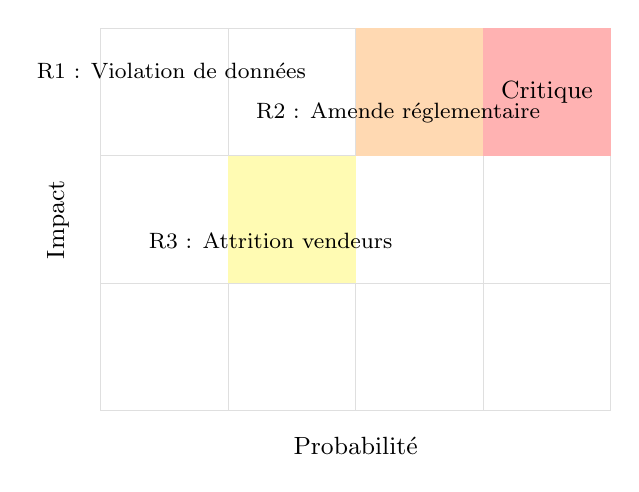
\begin{tikzpicture}[scale=0.9]
    \draw[step=1.8,gray!25] (0,0) grid (7.2,5.4);
    \node[rotate=90] at (-0.6,2.7) {\small Impact};
    \node at (3.6,-0.5) {\small Probabilité};
    \fill[red!30] (5.4,3.6) rectangle (7.2,5.4);
    \node[align=center,font=\small] at (6.3,4.5) {Critique};
    \fill[orange!30] (3.6,3.6) rectangle (5.4,5.4);
    \fill[yellow!30] (1.8,1.8) rectangle (3.6,3.6);
    \node[align=left,font=\footnotesize] at (1.0,4.8) {R1 : Violation de données};
    \node[align=left,font=\footnotesize] at (4.2,4.2) {R2 : Amende réglementaire};
    \node[align=left,font=\footnotesize] at (2.4,2.4) {R3 : Attrition vendeurs};
  \end{tikzpicture}
  \caption{Carte thermique illustrative des risques d'entreprise}
  \label{fig:risk-heatmap}
\end{figure}

\section{Gestion de la qualité}

Les objectifs de qualité comprennent l'exactitude des annonces, la réactivité du support et la cohérence des politiques. Les principes ISO 9001 informent la documentation des processus sans exiger une certification immédiate. Les boucles de retour client et le suivi du Net Promoter Score orientent les améliorations de service.

\section{Continuité des activités}

Les \gls{bcp} et \gls{drp} s'alignent sur les objectifs du chapitre sécurité. Les fonctions critiques---disponibilité de la plateforme, escalade de modération, communications de crise exécutives---disposent de priorités de reprise documentées. Des exercices de simulation ont lieu au moins annuellement.

\section{Indicateurs clés de performance}

Les KPI de gouvernance comprennent le taux de clôture des constats d'audit, l'actualité des revues de politiques, l'achèvement des formations et l'écart des coûts cloud par rapport au budget. Ils complètent les KPI commerciaux du chapitre~\ref{ch:business-vision}.

\section{Stratégie entrepreneuriale}

\subsection{Méthodologie Lean Startup}

MABRID applique des cycles Construire--Mesurer--Apprendre \parencite{ries2011lean} : formuler des hypothèses de proposition de valeur, lancer une présence minimale viable de place de marché dans les villes d'ancrage, mesurer l'engagement et les métriques de confiance, et pivoter ou persévérer sur la base des preuves.

\subsection{Adéquation produit-marché}

Les indicateurs d'adéquation produit-marché comprennent la croissance organique, la rétention élevée parmi les vendeurs ayant complété la vérification et les taux de recommandation par bouche-à-oreille. Les entretiens qualitatifs complètent les tableaux de bord quantitatifs.

\subsection{Stratégie de mise à l'échelle}

La mise à l'échelle procède géographiquement (déploiement par ville) et catégoriquement (profondeur verticale dans les secteurs à haute confiance). Un marketing national prématuré avant la liquidité locale risque une expérience utilisateur creuse.

\subsection{Avantage concurrentiel}

Un avantage durable découle de l'infrastructure de confiance---vérification, modération, communauté, posture de sécurité---coûteuse et lente à reproduire de manière crédible pour les concurrents \parencite{kim2005blueocean}.

\section{Conclusion du chapitre}

La gouvernance d'entreprise transforme MABRID d'un concept en organisation responsable. Des rôles clairs, une discipline des risques et une planification stratégique créent les conditions dans lesquelles les programmes de sécurité et juridiques (chapitres~\ref{ch:security} et~\ref{ch:legal}) peuvent fonctionner efficacement. Les investisseurs et partenaires devraient évaluer non seulement l'opportunité de marché, mais aussi la maturité des artefacts de gouvernance documentés dans le présent ouvrage.
